\documentclass[11pt,a4paper]{article}
\usepackage[T1]{fontenc}
\usepackage[utf8]{inputenc}
\usepackage{lmodern}
\usepackage{amsmath,amssymb,amsthm,mathtools,mathrsfs}
\usepackage{graphicx,float,xcolor,multicol}
\usepackage[shortlabels]{enumitem}
\usepackage[margin=27mm]{geometry}
\usepackage{microtype,needspace,placeins}
\usepackage{tikz,tikz-cd}
\usetikzlibrary{arrows.meta,calc,positioning,patterns,decorations.pathreplacing}
\usepackage[colorlinks=true,linkcolor=teal,urlcolor=teal,citecolor=teal]{hyperref}
\setlength{\parindent}{0pt}
\setlength{\parskip}{.6em}
\setcounter{secnumdepth}{0}
\allowdisplaybreaks
\raggedbottom
\providecommand{\cross}{\times}
\DeclareUnicodeCharacter{2020}{\ensuremath{\dagger}}
\DeclareMathOperator{\supp}{supp}
\DeclareMathOperator*{\esssup}{ess\,sup}
\providecommand{\chapter}{\section}
\newenvironment{tool}[2]{\subsection*{Tool #1 --- #2}}{}
\newcommand{\ToolRef}[1]{Tool #1}
\newcommand{\FigureTag}[2]{\textit{Figure #1}}
\newcommand{\Result}[1]{\subsection*{#1}}
\newcommand{\Application}[1]{\subsubsection*{Application\if\relax\detokenize{#1}\relax\else\space--- #1\fi}}
\newcommand{\ProofHeading}{\par\textit{Proof.}\space}
\newcommand{\ProofOf}[1]{\par\textit{Proof of #1.}\space}
\newcommand{\RemarkHeading}{\par\textbf{Remark.}\space}
\newcommand{\NoteHeading}{\par\textbf{Note.}\space}
\newcommand{\ExerciseHeading}{\par\textbf{Exercise.}\space}

\graphicspath{{figures/abels-theorem/}}
\begin{document}
\section*{Abel's Theorem}
% BLOG-CONTENT-BEGIN
\textbf{I)} \underline{\textbf{Prologue}}

Meromorphic functions are important tools in the theory of Riemann surfaces essentially because of the propositions below,

\subsection*{Proposition 0.1} The following are in bijective correspondence:-
\begin{itemize}
    \item $(n+1)$-linearly independent meromorphic functions on a compact Riemann surface $C$.
    \item non-degenerate holomorphic mappings $\phi: C\rightarrow \mathbb{CP}^n$.
\end{itemize}
where by non-degenerate we mean that $\phi(C)\not\subseteq \{z\in \mathbb{CP}^n |  L^i(z) = 0,  1\leq i\leq k,   \text{deg}(L^i) = 1\}$.


\subsection*{Proposition 0.2} Image of any non-degenerate holomorphic mapping $\phi:C\rightarrow \mathbb{CP}^2$ of a compact Riemann surface is an algebraic curve.

These convey that the set $\mathcal{M}(C)$ of meromorphic functions on $C$ acts as a bridge from Riemann surface theory to algebraic geometry: where Proposition $1$ sets up the scaffolding for projective embeddings, and Proposition $2$ paves way for algebraicity. Therefore, studying the existence of such functions is of relevance to us. In this regard, Abel's Theorem (stated below) provides systematic means of investigation. 

\subsection*{Theorem 0.3} Given a compact Riemann surface $C$ of genus $g$, there exists a $g$-dimensional complex torus $J(C)$, and a map, 
$$u:\text{Div}(C)^0 \rightarrow J(C)$$

such that $u(D) = 0$ if and only if $\exists$ $f\in \mathcal{M}(C)$ with $D = (f)$ (where $\text{Div}(C)^0$ is the collection of degree $0$ divisors of $C$). Further,
\begin{itemize}
    \item $J(C)$ is called the \textbf{Jacobian variety} of $C$.
    \item $u$ is called the \textbf{Abel-Jacobi map}.
\end{itemize}

Before setting up the construction of the Jacobian variety and proceeding further, let us acquaint ourselves with two important theorems. Let $C$ be a compact Riemann surface of genus $g$, $\Omega^1(C)$ the vector space of holomorphic $1$ forms on $C$ with basis $\omega_1, \ldots, \omega_g$, and $\mathcal{M}^1(C)$ the space of meromorphic differentials on $C$.

\textbf{II)} \underline{\textbf{Landmark Theorems}}

Recall, 

\begin{enumerate}[(i)]
    \item $C_{\bullet}^S(C) \hookrightarrow C_{\bullet}(C)$ is a quasi-isomorphism, where $C_{\bullet}(C)$ is the complex of singular simplices, and $C_{\bullet}^S(C)$ its subcomplex consisting of smooth singular simplices.
    \item $H_1(C, \mathbb{Z}) \cong \mathbb{Z}^{2g} \cong \langle \gamma_1, \ldots, \gamma_{2g}\rangle$, $\gamma_i$ smooth.
\end{enumerate}

By (i) and (ii), given any closed curve $\gamma$, we can replace it with, $$\widetilde{\gamma} = \sum_{i=1}^{2g}{n_i\gamma_i} + \partial \Omega \in C^S_1(C)$$ (where $\Omega \in C^S_2(C)$). Let $\lambda$ be a closed $1$ form on $C$, then, 
$$[\gamma] \in H_1(C, \mathbb{Z}) \xlongrightarrow{\pi_{\lambda}} \int_{\widetilde{\gamma}} \lambda \in \mathbb{C}$$

is well-defined. Indeed if $\gamma \sim \gamma'$ implies $\widetilde{\gamma} - \widetilde{\gamma'} = \partial \Omega$, and by Stokes' Theorem,
$$\int_{\widetilde{\gamma}}\lambda - \int_{\widetilde{\gamma'}}\lambda = \int_{\widetilde{\gamma} - \widetilde{\gamma'}}\lambda = \int_{\partial \Omega}\lambda = \iint_{\Omega}d\lambda = 0$$

here if $\Omega: \Delta^2 \rightarrow C$, then, $$\iint_{\Omega}d\lambda := \iint_{\Delta^2}\Omega^*(d\lambda)$$

Clearly, $\pi_{\lambda}$ is a group homomorphism. Also, if $\lambda \in H^1_{\text{dR}}(C, \mathbb{C})$, $\lambda \not\equiv 0$, $\pi_{\lambda}$ is non-trivial. For if it were trivial, 
$$\int_{\gamma_i}\lambda = 0  (1\leq i\leq 2g)$$

Fix $p_0\in C$ and set, 
$$f(p):= \int_{\gamma}\lambda$$

$\gamma(0) = p_0$, $\gamma(1) = p$, $\gamma$ a continuous path. To see that $f(p)$ is well-defined, let $\gamma'$ be another path with $\gamma'(0) = p_0$, $\gamma'(1) = p$, implies $\gamma - \gamma'$ is a $1$ cocycle,
$$\gamma - \gamma' = \sum_{i=1}^{2g}{n_i\gamma_i} + \partial \Omega$$

Stokes' theorem and the hypothesis settle further concerns. Now by Fundamental Theorem of Calculus, $df = \lambda$, which forces $\lambda \equiv 0$ (in $H^1_{\text{dR}}(C, 
\mathbb{C}))$. We therefore, have an injective homomorphism,
$$\pi: H^1_{\text{dR}}(C, \mathbb{C}) \rightarrow \text{Hom}(H_1(C, \mathbb{Z}), \mathbb{C})$$

Let $\overline{\Omega^1(C)} := \{\overline{\omega} |  \omega\in \Omega^1(C)\}$, and consider the map, 
$$\Omega^1(C)\bigoplus \overline{\Omega^1(C)} \rightarrow H^1_{\text{dR}}(C, \mathbb{C})$$
$$(\omega \oplus \overline{\phi}) \rightarrow \omega + \overline{\phi}$$

If $\omega + \overline{\phi} = df$, $f\in C^{\infty}(C)$, then, we shall show that $\omega = \phi = 0$. Suppose $\phi \not\equiv 0$, this implies locally $\phi = g(z)dz$, with $g(z) \not\equiv 0$. Note, 

$$\frac{i}{2}\phi\wedge \overline{\phi} = \frac{i}{2}|g(z)|^2dz\wedge d\overline{z} = |g(z)|^2dx\wedge dy$$
$$\implies   \frac{i}{2}\iint_C\phi\wedge\overline{\phi} = \iint_C|g(z)|^2dx\wedge dy >0$$

Also, 
$$\phi\wedge \overline{\phi} = \phi\wedge \omega + \phi\wedge \overline{\phi} = \phi\wedge(\omega+\overline{\phi}) = \phi\wedge df$$
$$d(f\phi) = df\wedge \phi + f\wedge d\phi = df\wedge \phi + 0$$

This implies, 
$$\iint_Cd(f\phi) = \iint_C\phi\wedge \overline{\phi} = 0$$

Contradiction. Clubbing our nuggets together, we have, 
$$\Omega^1(C)\bigoplus \overline{\Omega^1(C)} \hookrightarrow H^1_{\text{dR}}(C, \mathbb{C}) \hookrightarrow \text{Hom}(H_1(C, \mathbb{Z}), \mathbb{C})$$

Both $\text{Hom}(H_1(C, \mathbb{Z}), \mathbb{C})$ and $\Omega^1(C)\bigoplus \overline{\Omega^1(C)}$ are vector spaces of dimension $2g$, and, by Universal Coefficient Theorem, $\text{Hom}(H_1(C, \mathbb{Z}), \mathbb{C})\cong H^1(C, \mathbb{C})$. Therefore, in one shot we have, 

\begin{itemize}
    \item Hodge Theorem:- $\Omega^1(C)\bigoplus \overline{\Omega^1(C)} \cong H^1_{\text{dR}}(C, \mathbb{C})$ 
    \item De Rham Theorem:- $H^1_{\text{dR}}(C, \mathbb{C}) \cong H^1(C, \mathbb{C})$
\end{itemize}


\textbf{III)} \underline{\textbf{Jacobian Variety}}

\subsection*{Definition 0.1} Let $\gamma_1, \ldots, \gamma_{2g}$ be a basis for $H_1(C, \mathbb{Z})$, then,
$$a_{ij}:= \int_{\gamma_i}\omega_j$$

where $1\leq i \leq 2g,   1\leq j\leq g$ is called the \textbf{period matrix} of $C$.

\subsection*{Proposition 0.4}
    Columns of the period matrix are $\mathbb{R}$-linearly independent. 

\textit{Proof.} Suppose $\exists$ $c_i \in \mathbb{R}$ such that, 
$$c_1\int_{\gamma_1}\omega_i + \cdots c_{2g}\int_{\gamma_{2g}}\omega_i = 0$$
$$\implies c_1\int_{\gamma_1}\overline{\omega_i} + \cdots c_{2g}\int_{\gamma_{2g}}\overline{\omega_i} = 0$$

Consider the matrix, 
$$m_{ij} := \begin{cases}
a_{ij}, & 1\leq i \leq g\\
\overline{a_{ij}}, & g+1\leq i\leq 2g
\end{cases}$$

Clearly, rows of $m_{ij}$ are not $\mathbb{R}$-linearly independent. Therefore, we get real numbers $\mu_1, \ldots, \mu_g$ and $\nu_1, \ldots, \nu_g$, such that, 
$$\int_{\gamma_j} \Bigg(\sum_{i=1}^{g}{\mu_i\omega_i} + \sum_{i=1}^{g}{\nu_i\overline{\omega_i}} 
  \Bigg) = 0   (1\leq j\leq 2g)$$
  
  Set, $$\omega = \sum_{i=1}^{g}{\mu_i\omega_i}, \text{ and } \phi = \sum_{i=1}^{g}{\nu_i\omega_i}$$
  
  By De Rham Theorem, $\omega + \overline{\phi} = 0$, and by Hodge Theorem $\omega = \phi = 0$. Contradiction.

Therefore, $\{a_{ij}\}$ forms a lattice. Set $\Lambda$ to be the lattice generated by $\{a_{ij}\}$, then $\Lambda$ acts on $\mathbb{C}^g$ via translations, which is both free and properly discontinuous. Define, 
$$J(C):= \mathbb{C}^g/\Lambda$$

a $g$-dimensional complex torus. Now, the litmus test Abel's Theorem provides for when meromorphic functions with prescribed poles and zeroes can exist relies on the Abel-Jacobi map, which we now describe. Fix $q\in C$,
$$u: \text{Div}(C)^0 \rightarrow J(C)$$
$$u\bigg(\sum_{i}{n_ip_i}\bigg) := \Bigg(\sum_{i}{n_i\int_{q}^{p_i}\omega_j}\Bigg)_{1\leq j\leq g}$$

This is well-defined because for different choices of paths from $q$ to $p_i$, the differences between the associated Abel-Jacobi maps lie in $\Lambda$. 

\textbf{IV)} \underline{\textbf{Proof of Abel's Theorem}}

Note that to prove Abel's Theorem we have to show that the following sequence is exact:-
$$\mathcal{M}(C)^* \xrightarrow{(\cdot)} \text{Div}(C)^0 \xrightarrow{u} J(C)$$

where $(\cdot)$ is the function that sends $f$ to $(f)$, and $\mathcal{M}(C)^*$ is the set of all non-zero meromorphic functions on $C$. We shall prove the above in two parts: (i) $\text{Im}\big((\cdot)\big) \subseteq \text{Ker}(u)$, and (ii) $\text{Ker}(u) \subseteq \text{Im}\big((\cdot)\big)$. 

\underline{Proof of (i)}:- Let $f \in \mathcal{M}(C)^*$. $f$ can be seen as a ramified cover of $\mathbb{CP}^1$. For $t\in \mathbb{CP}^1$, let $\{p_i(t)\}_{1\leq i\leq n} = f^{-1}(t)$ with ramification indices $\{n_i\}_{1\leq i\leq n}$. Then set, $$D_t:= \sum_{i=1}^{n}{n_ip_i(t)} \in \text{Div}(C)$$

We shall begin by showing that $u(D_t)$ is holomorphic in $t$. Let $t_0\in \mathbb{CP}^1\backslash \{\infty\}$ be a point that's not branched by $f$, then one can find disks $\mathbb{D}_{p_j(t_0)}$ around $p_j(t_0)$ and a disk $\mathbb{D}_{t_0}$ around $t_0$ such that,
$$f:\mathbb{D}_{p_j(t_0)}\rightarrow \mathbb{D}_{t_0}$$

is a biholomorphism. Viewing $\mathbb{CP}^1$ as $\mathbb{C} \cup \{\infty\}$, let $f$ be the local coordinate for $\mathbb{D}_{p_j(t_0)}$, and suppose that with respect those coordinates on $\mathbb{D}_{p_j(t_0)}$,
$$\omega_i \equiv h_{ij}(z)dz$$

Then for $t \in \mathbb{D}_{p_j(t_0)}$, $1\leq j\leq n$,
$$\int_{q}^{p_j(t)}\omega_i = \int_{q}^{p_j(t_0)}\omega_i + \int_{p_j(t_0)}^{p_j(t)}\omega_i = \int_{q}^{p_j(t_0)}\omega_i + \int_{t_0}^{t}h_{ij}(z)dz$$

Now by Fundamental Theorem of Calculus, 
$$\frac{d}{dt}\int_{t_0}^{t}h_{ij}(z)dz = h_{ij}(t) = (2\pi i)\cdot\text{Res}_t\bigg(\frac{h_{ij}(z)dz}{z-t}\bigg)$$

By definition, 
$$(2\pi i)\cdot\text{Res}_t\bigg(\frac{h_{ij}(z)dz}{z-t}\bigg) = (2\pi i)\cdot\text{Res}_{p_j(t)}\bigg(\frac{w_i}{f-t}\bigg)$$

Residue Theorem further yields,

$$\frac{d}{dt}\sum_{j=1}^{n}{\int_{q}^{p_j(t)}\omega_i} = (2\pi i)\cdot \sum_{j=1}^{n}{\text{Res}_{p_j(t)}\bigg(\frac{w_i}{f-t}\bigg)} = 0$$

Let $B$ denote the set of branch points of $f$ along with $\{\infty\}$, then on $\mathbb{CP}^1\backslash B$, $u(D_t)$ is holomorphic. And as $\mathbb{CP}^1\backslash B$ is connected, $u(D_t)$ is constant. Now, by Riemann Removable Singularity Theorem,
$$u(D_t) = c_0   (t \in \mathbb{CP}^1)$$

Therefore, 
$$u((f)) = u(D_0) - u(D_{\infty}) = 0$$

thereby proving (i).
\qed

\underline{Proof of (ii)}:- Let us forget (for a while) everything about the Abel-Jacobi map and focus on the question of existence of a certain type of meromorphic function. We shall begin this venture by shifting the burden of constructing specific meromorphic functions to constructing specific forms. Because once we have forms, we can procure a meromorphic function by integrating it suitably (as shall be demonstrated soon). Proceeding in this direction, we have the following theorem,

\subsection*{Theorem 0.5} Given $p, q \in C$, there exists meromorphic differential $\phi$ with poles only at $p$ and $q$ of order $1$.


\textit{Proof.}
    By applying Riemann-Roch Theorem to the divisor $D = -(p+q)$, we have,
    $$l(D) - i(D) = \text{deg}(D) + 1 - g = -(g+1)$$
    
    Now, as there can be no vanishing holomorphic function on a compact Riemann surface, $l(D) = 0$, forcing $i(D) = g+1$, which exceeds the dimension of the space of holomorphic $1$ forms on $C$. This yields a meromorphic form $\phi$ with a simple pole either on $p$ or $q$. WLOG, assume $\phi$ has a simple pole at $p$, then $\text{Res}_p(\phi) \neq 0$, and Residue Theorem forces $\text{Res}_q(\phi) \neq 0$. Therefore, $\phi$ is our desired differential.

\textbf{Remark.} Let $D = (p_1 +\cdots + p_n) - (q_1 +\cdots + q_n) \in \text{Div}(C)^0$. Then, one can construct meromorphic differentials with simple poles at $\{p_i, q_i\}_{1\leq i\leq n}$ by summing up differentials with simple poles at $p_i$ and $q_i$ obtained in the theorem above. Further, by multiplying $\phi$ in the preceding theorem by a suitable constant one can ensure that, $$\text{Res}_{p_i}(\phi) = \frac{1}{2\pi i}, \text{ and } \text{Res}_{q_i}(\phi) = \frac{-1}{2\pi i}$$
In summary, one can arrange for a differential $\phi$ corresponding to $D = \sum_jn_jp_j \in \text{Div}(C)^0$ satisfying:-
\begin{itemize}
    \item $\phi$ only has simple poles, and they are at points $\{p_j\}_j$.
    \item $\text{Res}_{p_j}(\phi) = \frac{n_j}{2\pi i}$
\end{itemize}


\textbf{Construction.} Fix $q\in C$, and consider the differential $\phi$ given above for a divisor $D \in \text{Div}(C)^0$ and define (if you can),
$$f(p) := \text{exp}\bigg(2\pi i\int_{q}^{p}\phi\bigg)$$

Again, Fundamental Theorem of Calculus would ensure that $f$ is holomorphic and non-vanishing everywhere but at points $\{p_i\}_i$. Suppose $(\mathbb{D}_{p_j}, z)$ is a local coordinate chart centered at a point $p_j$. Then,

$$\phi \equiv \bigg(\frac{n_i}{2\pi i}\bigg)\frac{dz}{z} + h(z)dz$$

where $h(z)$ is holomorphic. Fix a point $p_0 \neq p_i$ in $\mathbb{D}_{p_j}$, and suppose $z(p_0) = z_0$, then,


\begin{equation*}
    \begin{aligned}
        f(z) &= \text{exp}\bigg(2\pi i\int_{q}^{p}\phi\bigg)\\
            &= \text{exp}\bigg(2\pi i\bigg(\int_{q}^{p_0}\phi + \int_{p_0}^{p}\phi\bigg)\bigg)\\
            &= \text{exp}\bigg(2\pi i\bigg(\int_{q}^{p_0}\phi + \int_{z_0}^{z}{\frac{n_i}{2\pi i}\frac{dz}{z}} + \int_{z_0}^{z}h(z)dz\bigg)\bigg)\\
            &= \text{exp}\bigg(2\pi i\bigg(\int_{q}^{p_0}\phi - \frac{n_i}{2\pi i}\text{ln}z_0 + \frac{n_i}{2\pi i}\text{ln}z + \int_{z_0}^{z}h(z)dz\bigg)\bigg)\\
            &= cz^{n_i}H(z)
    \end{aligned}
\end{equation*}

where, 
$$c = \text{exp}\bigg(2\pi i\bigg(\int_{q}^{p_0}\phi - \frac{n_i}{2\pi i}\text{ln}z_0 \bigg)\bigg)$$

is a non-zero constant and,
$$H(z) = \text{exp}\bigg(2\pi i \int_{z_0}^{z}h(z)dz\bigg)$$

is a non-vanishing holomorphic function. Hence, 
$$(f) = \sum_{i}n_ip_i = D$$

We could have concluded right now had there been no issue with the way $f$ is defined. But unfortunately, $f$ is not always well-defined. Suppose there are two paths $\gamma$ and $\gamma'$ connecting $q$ and $p$, then,
$$\text{exp}\bigg(2\pi i\int_{\gamma}\phi\bigg) = \text{exp}\bigg(2\pi i\int_{\gamma'}\phi\bigg)$$

if and only if,
$$\bigg(\int_{\gamma}\phi - \int_{\gamma'}\phi\bigg) \in \mathbb{Z}$$

So, apart from the two conditions that a differential in the Remark above can be made to satisfy, if it were to also satisfy,
$$\bigg(\int_{\gamma_j}\phi\bigg) \in \mathbb{Z}   (1\leq j \leq 2g)$$

where $\gamma_j$ are the smooth $1$-cocycles spanning $H^1(C, \mathbb{Z})$, then, the construction above resolves (ii) entirely. Therefore, we shall take a detour to invest our minds in analyzing the newly introduced hypothesis.

\textbf{V)} \underline{\textbf{Riemann's Bilinear Relations}}

If a differential $\phi$ satisfies the two conditions spelled out in the Remark above, then so does $\phi + \omega$, for any $\omega \in \Omega^1(C)$. So, our strategy would be to look for a suitable $\omega \in \Omega^1(C)$ such that $\phi + \omega$ satisfies the additional hypothesis. This naturally leads us to study the functionals defined below,
$$\pi_i: \Omega^1(C) \rightarrow \mathbb{C}$$
$$\pi_i(\omega):= \int_{\gamma_i}\omega$$

where $\gamma_i$ is a distinguished homology basis for $C$ described in Figure 1.
\begin{figure}[htp]
            \centering
        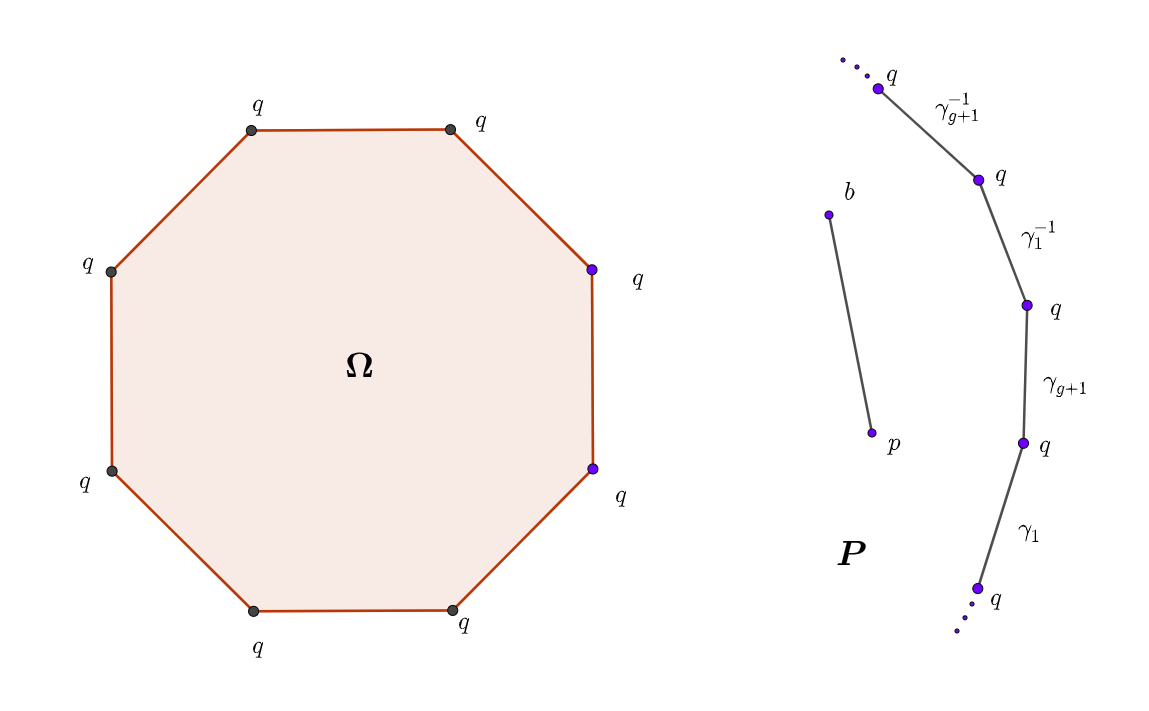
\includegraphics[width=15cm]{Polygon.png}
            \caption{$P$ is the polygonal representation of $C$. The distinguished homology basis of $C$ is shown along the boundary of $P$.}
        \end{figure}

The integrals associated to $\omega$ above are called its \textbf{periods}. Turns out that these functionals naturally satisfy certain bilinear relations, recorded in the theorem below,

\subsection*{Theorem 0.6}
    For any $\omega, \phi \in \Omega^1(C)$, we have,
    $$\sum_{i=1}^{g}\big(\pi_i(\omega)\pi_{g+i}(\phi) - \pi_{g+i}(\omega)\pi_i(\phi)\big) = 0$$
    $$\sqrt{-1} \sum_{i=1}^{g}\big(\pi_i(\omega)\overline{\pi_{g+i}(\phi)} - \pi_{g+i}(\omega)\overline{\pi_i(\phi)}\big) > 0$$

\textit{Proof.}

    Set, 
    $$\Omega := C - \bigcup_{i = 1}^{2g} \gamma_i$$

Fix a point $b\in \Omega$, and define, 
$$A(p):= \int_{b}^{p}\omega$$

where $p \in \Omega$. As $\Omega$ is simply connected, any two paths between $b$ and $p$ will be homotopic, thereby making $A$ into a well-defined single-valued function which by Fundamental Theorem of Calculus is holomorphic. As derivatives of $A$ extend to $P$ locally, so will its primitives, which by identity theorem is $A$ on $\Omega$. In other words, $A$ extends to $P$, which implies $A\phi \in \Omega^1(P)$. The letter $\Omega$ shall also be used to represent the 2-cycle which in this case is the characteristic map $(\Omega: P \rightarrow C)$ of the CW-complex structure on $C$. Further, on $P$ we have, 
$$d(A\phi) = dA\wedge \phi + Ad\phi = \omega\wedge\phi + 0 = 0$$

which goes to show that $A\phi$ is a closed $1$ form. By Stokes' Theorem on the $2$-cycle $\Omega$, we have,
$$\int_{\partial\Omega}A\phi = 0$$
Also, 
$$\int_{\partial\Omega}A\phi = \sum_{i=1}^{g}\bigg(\int_{\gamma_i}A\phi + \int_{\gamma_{g+i}}A\phi + \int_{\gamma_i^{-1}}A\phi + \int_{\gamma_{g+i}^{-1}}A\phi\bigg)$$
upon clubbing $\gamma_i$ and $\gamma_i^{-1}$, we get, 
$$\int_{\gamma_i}A\phi + \int_{\gamma_i^{-1}}A\phi = \int_{\gamma_i}(A(p) - A(p'))\phi$$

where $p$ and $p'$ represent the same point on $\gamma_i$ and $\gamma_i^{-1}$, and the minus sign is due to the change in orientation of $\gamma_i$. We know,

$$A(p) - A(p') = \int_{p}^{p'}\omega = \int_{p'}^{q}\omega - \int_{\gamma_{g+i}}\omega + \int_{q}^{p}\omega = -\pi_{g+i}(\omega)$$

Putting it together we have,
$$\int_{\gamma_i}A\phi + \int_{\gamma_i^{-1}}A\phi = -\pi_{g+i}(\omega)\pi_{i}(\phi)$$

and similarly, 
$$\int_{\gamma_{g+i}}A\phi + \int_{\gamma_{g+i}^{-1}}A\phi = \pi_{i}(\omega)\pi_{g+i}(\phi)$$

In conjunction, they yield the first identity. Now note,
$$d(\sqrt{-1}A\overline{\omega}) = \sqrt{-1}(dA\wedge \omega + Ad\overline{\omega}) = \sqrt{-1}\omega\wedge\overline{\omega}$$

which yields, 
$$\sqrt{-1}\int_{\partial\Omega}A\overline{\omega} = \sqrt{-1}\iint_{\Omega}\omega\wedge\overline{\omega} > 0$$

and proceed similarly as before to compute,
$$\sqrt{-1}\int_{\partial\Omega}A\overline{\omega}$$

to arrive at the second identity. 

\textbf{Remark.} Let $\Pi = (A_{g\times g}, B_{g\times g})$ be the period matrix of $C$. Let coordinates of $w = (w_1,\ldots,w_{2g})$ be the periods of $\omega$ and that of $v = (v_1,\ldots,v_{2g})$ be the periods of $\phi$, and let,
$$Q = \begin{pmatrix} 0&\text{Id}_{g\times g}\\-\text{Id}_{g\times g}&0
\end{pmatrix}$$

Note that, the identities in the theorem above can be rewritten as
$$wQv^T = 0$$
$$wQ\overline{w}^T > 0$$
If $\omega = \sum_{1\leq i\leq g}\mu_i\omega_i$, and $\phi = \sum_{1\leq i\leq g}\nu_i\omega_i$, then the above can be rewritten as,
$$\big((\mu_1,\ldots, \mu_g)\big(\Pi Q\Pi^T\big)(\nu_1, \ldots, \nu_g)^T = 0\big) \iff \big(\Pi Q\Pi^T = 0\big)$$
$$\big(\sqrt{-1}(\mu_1,\ldots, \mu_g)\big(\Pi Q\overline{\Pi}^T\big)(\overline{\mu}_1, \ldots, \overline{\mu}_g)^T > 0\big) \iff \big(\sqrt{-1}\Pi Q\overline{\Pi}^T \text{ is a positive definite Hermitian matrix}\big)$$

Therefore, Riemann's Bilinear Relations is equivalent to the following compressed assertions:-
\begin{enumerate}[(a)]
    \item $A^TB = B^TA$
    \item $\sqrt{-1}(A^T\overline{B} - B^T\overline{A}) \text{ is a positive definite Hermitian matrix}$.
\end{enumerate}

One immediately sees that (b) implies $A$ is non-singular. Transforming the basis of $\Omega^1(C)$ by $(A^{-1})^T$ would yield the following simple form for the period matrix,
$$\Pi = (\text{Id}_{g\times g}, Z_{g\times g})$$

which is often referred to as the \textbf{normalized period matrix} of $C$.

\underline{Completion of the Proof of (ii)}:- Let $\phi$ be the differential corresponding to $(p_1+\cdots+p_n) - (q_1+\cdots+q_n) = D \in \text{Div}(C)^0$. Let $\gamma_i$ be the distinguished homology basis as before and let none of them pass through the poles of $\phi$. Let $\omega_1, \ldots, \omega_g$ be a basis of $\Omega^1(C)$ such that the corresponding period matrix is normalized. Let,

$$\phi' = \phi - \sum_{j=1}^{g}\bigg(\int_{\gamma_j}\phi\bigg)\omega_j$$

Poles and residues of $\phi'$ and $\phi$ are the same, and,
$$\int_{\gamma_i}\phi' = \int_{\gamma_i}\phi - \sum_{j=1}^{g}\pi_j(\phi)\pi_i(\omega_j) = \int_{\gamma_i}\phi - \int_{\gamma_i}\phi = 0$$

We shall borrow $\Omega$ and $A$ from the proof of Riemann's Bilinear Relations. Now by Residue Theorem, we get, 
$$2\pi \sqrt{-1}\sum_{j=1}^{n}\big(\text{Res}_{p_j}(A\phi') + \text{Res}_{q_j}(A\phi')\big) =  \int_{\partial\Omega}A\phi'$$

LHS of the above can be rewritten as, 
$$\sum_{j=1}^{n}(A(p_j) - A(q_j)) = \sum_{j=1}^{n}\int_{q_j}^{p_j}\omega$$

and the RHS can be rewritten like in the proof of Theorem 0.6 as, 
$$\int_{\partial\Omega}A\phi' = \sum_{i=1}^{g}(\pi_i(\omega)\pi_{g+i}(\phi') - \pi_{g+i}(\omega)\pi_i(\phi'))$$

By the fact that $\pi_j(\phi') = 0$ for $1\leq j\leq g$, we get, 
$$\int_{\partial\Omega}A\phi' = \sum_{i=1}^{g}\pi_i(\omega)\pi_{g+i}(\phi')$$

Clubbing the previous three equations for $\omega = \omega_i$,
$$\sum_{j=1}^{n}\int_{q_j}^{p_j}\omega_i = \sum_{j=1}^{n}\pi_j(\omega_i)\pi_{g+j}(\phi')$$

which yields, 
$$\sum_{j=1}^{n}\int_{q_j}^{p_j}\omega_i = \pi_{g+i}(\phi')   (\dagger)$$

Now, let us suppose that $u(D) = 0$, then for $1\leq i\leq g$,
\begin{center}
\begin{equation*}
        \begin{aligned}
            \sum_{j=1}^{n}\int_{q_j}^{p_j}\omega_i &= \bigg(\sum_{j=1}^{2g}m_j\int_{\gamma_j}\omega_i\bigg) \in \Lambda \\
            &= \sum_{j=1}^{g}\bigg(m_j\int_{\gamma_j}\omega_i + m_{g+j}\int_{\gamma_{g+j}}\omega_i\bigg)\\
            &= m_i + \sum_{j=1}^{g} m_{g+j}\int_{\gamma_{g+j}}\omega_i
        \end{aligned}
\end{equation*}
\end{center}

$\Pi = (\text{Id}, Z)$ being the period matrix for $C$ satisfies $Z = Z^T$, which means, 
$$\int_{\gamma_{g+j}}\omega_i = \int_{\gamma_{g+i}}\omega_j$$

and thus, 
$$\sum_{j=1}^{n}\int_{q_j}^{p_j}\omega_i = m_i + \sum_{j=1}^{g} m_{g+j}\int_{\gamma_{g+i}}\omega_j$$

By $(\dagger)$ we get,
$$\pi_{g+i}(\phi') = m_i + \sum_{j=1}^{g} m_{g+j}\int_{\gamma_{g+i}}\omega_j   (\dagger\dagger)$$

Now let, 
$$\widetilde{\phi}:= \phi' - \sum_{j=1}^{g} m_{g+j}\omega_j$$

and note that as $\pi_j(\omega_i) = \delta_{ij}$ for $i,j = 1, \ldots, g$, we have,

$$\int_{\gamma_i}\widetilde{\phi} = \int_{\gamma_i}\phi' - \sum_{j=1}^{g} m_{g+j}\omega_j = -m_{g+i} \in \mathbb{Z}$$

and by $(\dagger\dagger)$,
$$\int_{\gamma_{g+i}}\widetilde{\phi} = \pi_{g+i}(\phi') - \sum_{j=1}^{g} m_{g+j}\int_{\gamma_{g+i}}\omega_j = m_i \in \mathbb{Z}$$

In conclusion, $\widetilde{\phi}$ is the differential that would make our construction work and settle the proof of (ii) once and for all. 
\qed

\textbf{Remark.} The relevance of Abel's Theorem to the existence of meromorphic functions is that the Abel-Jacobi map is surjective (which is often referred to as Jacobi's Inversion Theorem).
% BLOG-CONTENT-END
\end{document}
